\section{HACER-RAG System Architecture}
\label{sec:architecture}

\begin{figure*}[t]
\centering
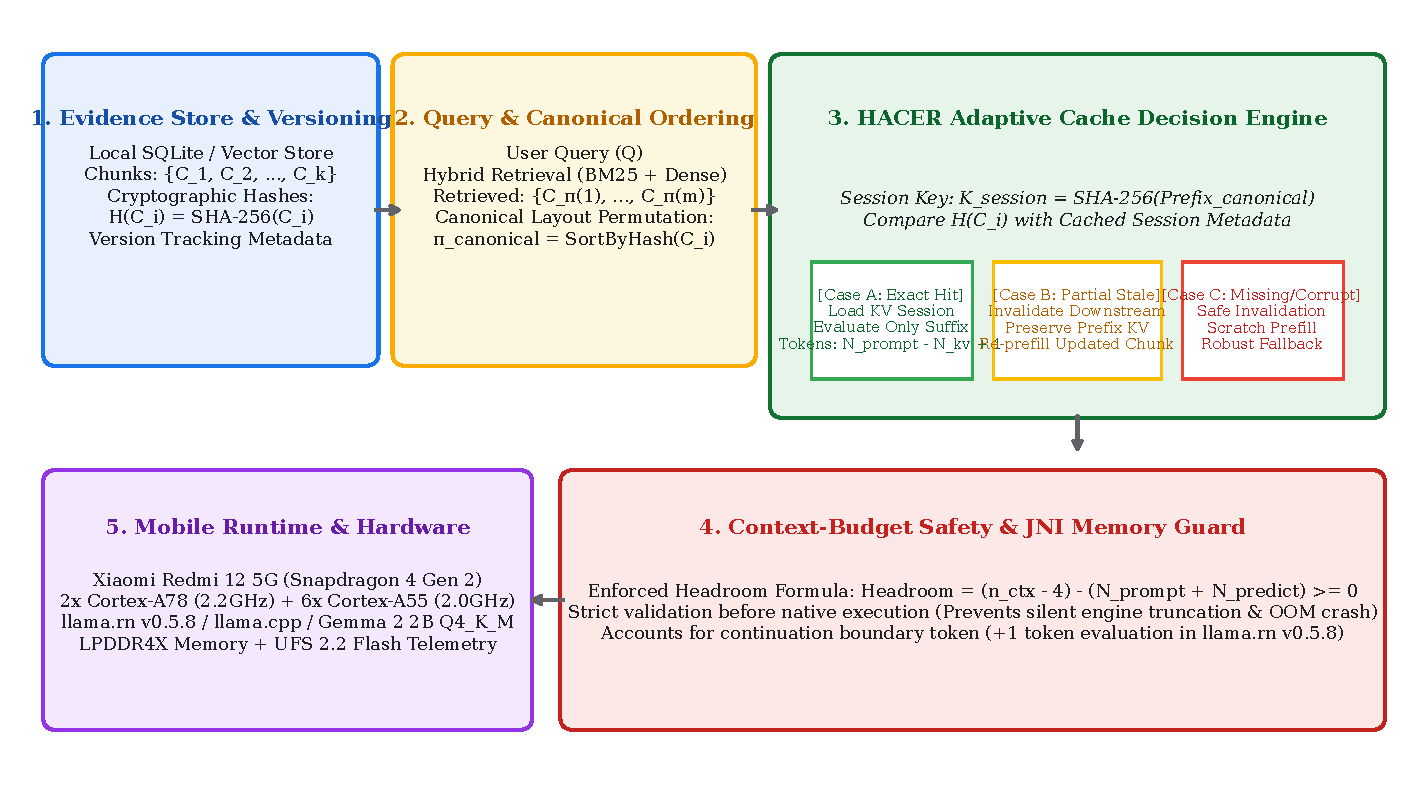
\includegraphics[width=\textwidth]{figures/fig1_system_architecture.pdf}
\caption{\textbf{The HACER-RAG Mobile Inference Architecture.} The system coordinates: (1) local evidence chunk versioning with cryptographic SHA-256 hashes; (2) hybrid retrieval with canonical layout ordering; (3) an adaptive cache decision engine that classifies requests into exact prefix hits, selective downstream repair, or safe scratch fallback; (4) JNI-level context-budget safety and continuation boundary-token alignment; and (5) native execution via \texttt{llama.rn}/\texttt{llama.cpp} with hardware telemetry profiling.}
\label{fig:architecture}
\end{figure*}

The architecture of HACER-RAG is illustrated in Figure~\ref{fig:architecture}. It comprises five tightly integrated subsystems: (1) Evidence Ingestion and Version Tracking; (2) Canonical Retrieval and Layout; (3) Adaptive Cache Decision Engine; (4) Context-Budget Safety Guard; and (5) Native Execution and Telemetry Profiler.

\subsection{Evidence Ingestion and Version Tracking}
In an on-device personal knowledge base, text documents (e.g., policy documents, notes, manuals) are partitioned into discrete chunks $\mathcal{C} = \{C_1, C_2, \dots, C_M\}$. Unlike conventional mobile vector databases that store only text strings and embedding vectors, HACER-RAG computes and maintains a cryptographic digest for each chunk:
\begin{equation}
    H(C_i) = \text{SHA-256}(\text{Canonicalize}(C_i))
\end{equation}
This cryptographic digest is persisted in an on-device SQLite database alongside the chunk's creation timestamp, unique document ID, and token count. Any modification, deletion, or addition to a document produces an immediate mismatch in $H(C_i)$.

\subsection{Canonical Evidence Layout}
A major challenge in multi-chunk RAG caching is the \emph{chunk permutation problem}. Given $k$ retrieved chunks relevant to a query, standard retrievers return chunks ranked by relevance score. If relevance scores fluctuate slightly across subsequent queries, the retriever may return permutations such as $[C_2, C_1]$ instead of $[C_1, C_2]$. 

In causal attention mechanisms, exchanging the positions of $C_1$ and $C_2$ alters the entire token sequence, rendering any previously saved prefix KV cache useless ($0\%$ reuse). HACER-RAG addresses this by enforcing a \emph{Canonical Evidence Layout}. When $k$ chunks are selected for prompt construction, HACER-RAG groups the chunks and applies a deterministic ordering policy:
\begin{equation}
    \pi_{\text{canonical}} = \text{Sort}(\{C_1, \dots, C_k\})
\end{equation}
By sorting chunks according to their persistent document and chunk identifiers, the textual prefix prefix sequence is stabilized across queries, maximizing exact prefix cache hits regardless of minor variations in retriever ranking scores.

\subsection{The Adaptive Cache Decision Engine}
When a user issues query $Q$, the system constructs the candidate prompt prefix from the canonically ordered retrieved chunks:
\begin{equation}
    P = \text{FormatPrompt}(\pi_{\text{canonical}}(\{C_1, \dots, C_k\}))
\end{equation}
The engine computes the composite prefix hash:
\begin{equation}
    \mathcal{K}_{\text{session}} = \text{SHA-256}(P)
\end{equation}
The Decision Engine inspects local flash storage for an active session binary matching $\mathcal{K}_{\text{session}}$ and determines the execution strategy:
\begin{enumerate}
    \item \textbf{Case 1 (Exact Prefix Hit):} A valid session file matching $\mathcal{K}_{\text{session}}$ exists, and all underlying chunk hashes $H(C_i)$ match current corpus state. The engine instructs the native runtime to load the KV session from flash. Only the query suffix $Q$ is evaluated online.
    \item \textbf{Case 2 (Selective Downstream Repair):} A partial prefix match exists (e.g., chunks $C_1, \dots, C_{j}$ are unchanged, but chunk $C_{j+1}$ was modified or newly inserted). The engine loads the prefix KV cache up to chunk $C_j$, preserves the valid resident KV tensors, and triggers online prefill exclusively for the modified chunk $C_{j+1}$ and query $Q$.
    \item \textbf{Case 3 (Safe Invalidation and Scratch Fallback):} If a document chunk was revoked/deleted, or if the session binary is corrupted, missing, or fails size/header validation, the engine invalidates the cached session, purges orphaned cache files, and initiates clean scratch prefill from token position 0.
\end{enumerate}

\subsection{Native Execution and Telemetry Profiler}
The execution layer interfaces with \texttt{llama.rn} (v0.5.8), a React Native JNI wrapper around \texttt{llama.cpp}. HACER-RAG intercepts native execution to collect granular systems telemetry:
\begin{itemize}
    \item \textbf{Kernel I/O Instrumentation:} Polling Linux kernel counters via \texttt{/proc/\{PID\}/io} before and after execution to measure exact physical storage bytes read (\texttt{read\_bytes}), write bytes (\texttt{write\_bytes}), and I/O system calls (\texttt{syscr}, \texttt{syscw}). This enables separating physical UFS 2.2 flash reads from Linux page-cache hits.
    \item \textbf{Memory Footprint:} Capturing Android Total Proportional Set Size (PSS) via \texttt{dumpsys meminfo} to detect memory expansion and prevent LMK eviction.
    \item \textbf{SoC Telemetry:} Monitoring battery temperature and CPU clock frequencies via Android sysfs to account for thermal throttling across repeated benchmark runs.
\end{itemize}
